\textbf{Newman's Convergence Theorem} \\
$\sum\frac{f(n)}{n^z}$, $\abs{f(n)}\leq1$
\[ \myvcenter{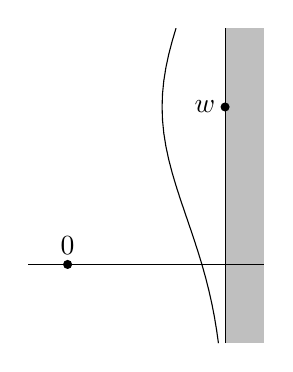
\begin{tikzpicture}[scale=2]
\path[fill=lightgray](1,1.5)--(1,-0.5)--(1.25,-0.5)--(1.25,1.5)--cycle;
\begin{scope}[shift={(1,1)}]
\draw[domain=-1.5:0.5]plot({1-exp(-\x*\x)/2.5-1},\x);
\end{scope}
\draw(-0.25,0)--(1.25,0);
\draw(1,-0.5)--(1,1.5);
\draw[fill](0,0)circle(0.025);
\draw[fill](1,1)circle(0.025);
\node[above]at(0,0){$0$};
\node[left]at(1,1){$w$};
\end{tikzpicture}}
\qquad\qquad
\myvcenter{\begin{tikzpicture}[scale=2]
\path[fill=lightgray](100:0.3)--(-100:0.3)arc(-100:100:0.3);
\draw(-0.5,0)--(0.5,0);
\draw(0,-0.5)--(0,0.5);
\draw[domain=-0.75:0.75]plot({1-exp(-\x*\x)/2.5-1},\x);
\draw[decoration={markings,mark=at position 0.25 with {\arrow{>},\node[left]{$\beta$};}},postaction=decorate](100:0.3)--(-100:0.3);
\draw[decoration={markings,mark=at position 0.666 with {\arrow{>},\node[above]{$\alpha$};}},postaction=decorate](-100:0.3)arc(-100:100:0.3);
\end{tikzpicture}} \]
\begin{gather*}
S_l(w)=\sum_{n=1}^\infty\frac{f(n)}{n^w} \\
\int_\gamma F(w+z)l^z\paren[\big]{\frac1z+\frac z{R^2}} \\
2\pi i(F(w)-S_l(w)) = A + B \\
A = \int_\alpha(E_l(w+z)l^z-S_l(w-z)l^{-z})\parenBig{\frac1z+\frac z{R^2}}\d z \\
A \leq \frac{?}{R} + \frac{?}{l} \\
B = \int_\beta F(w+z) l^z \parenBig{\frac1z+\frac z{R^2}}\d z
\end{gather*}
%
%\[ B = \int_\beta F(w+z)l^z\parenBig{\frac1z+\frac z{R^2}}\d z \]
for $z$ on $\beta$ with $\abs{z}=R$
\[ \absBig{\frac1z+\frac z{R^2}} = \absBig{\frac{\overline z+z}{R^2}} = \absBig{\frac{2x}{R^2}} = \frac{-2x}{R^2} \]
where $x=\Re(z)$, also $\beta$ can be given by
\begin{align*}
\beta(t) &= -t\pm i\sqrt{R^2-t^2}\co0\leq t\leq r \\
\beta'(t) &= -1\pm i\frac{t}{\sqrt{R^2-t^2}} \\
\abs{\beta'(t)}^2 &= 1 + \frac{t^2}{R^2-t^2} = \frac{R^2}{R^2-t^2} \leq \frac{R^2}{R^2-r^2} \leq \frac{1}{1-\frac14}
\end{align*}
for $z$ with $\Re(z)=-r$
\[ \absBig{\frac1z+\frac z{R^2}} = \absBig{\frac1z\parenBig{1+\frac{z^2}{R^2}}} \leq \frac1r\parenBig{1+\frac{R^2}{R^2}} = \frac{2}{r} \]
\begin{align*}
\therefore \abs{B} &\leq 2\int_0^r M\cdot l^{-t}\cdot\frac{2t}{R^2}\cdot N\d t + 2RMl^{-r}\frac{2}{r} \\ \intertext{where $M=\max_{\text{$z$ on $\beta$}}\abs{F(w+z)}$, $N=\max_{0\leq t\leq r}\abs{\beta'(t)}\leq\frac{2}{\sqrt3}$}
&= \frac{4MN}{R^2} \int_0^r \frac{t}{l^t} \d t + \frac{4RM}{rl^r} \\
&= \frac{4MN}{R^2} \brackBig{-\frac{t}{\log l\cdot l^t}-\frac{1}{(\log l)^2l^t}}_0^r + \frac{4RM}{rl^r}\footnote{
\[ \int \underbrace{t}_u \underbrace{l^{-t}\d t}_{\!\d v} = \frac{-t}{\log l\cdot l^t} + \int\frac{l^{-t}}{\log l} \]
$\!\d v=e^{-t\log l}$, $v=-\frac1{\log l}l^{-t}$} \\
&\leq \frac{4MN}{R^2(\log l)^2} + \frac{4RM}{rl^r} \to 0 \text{ as $l\to\infty$}
\end{align*}
\thm (Prime Number Theorem)
\begin{enumerate}
\item $\sum_{n=1}^\infty\frac{\mu(n)}{n}=0$
\item $\sum_{n\leq x}\mu(n)=o(x)$, i.e., $\lim_{x\to\infty}\frac1x\sum_{n\leq x}\mu(n)=0$
\item $\psi(x)\sim x$, i.e., $\lim_{x\to\infty}\frac{\psi(x)}{x}=1$ where $\psi(x)=\sum_{n\leq x}\Lambda(n)=\sum_{p^k\leq x}\log(p)$
\item $\vartheta(x)\sim x$, i.e., $\lim_{x\to\infty}\frac{\vartheta(x)}{x}=1$ where $\vartheta(x)=\sum_{p\leq x}\log p$
\item $\pi(x)\sim\frac{x}{\log x}$, i.e., $\lim_{x\to\infty}\frac{\pi(x)\log x}{x}=1$ where $\pi(x)=\sum_{p\leq x}1=\sum_{n\leq x}\rho(n)$
\item $p_n=p(n)\sim n\log n$ where $\rho(n)$ is the $n$th prime.
\end{enumerate}
\pf \textbf{NCT}$\implies$(1) \\
For $\Re(z)>1$, $\zeta(z)M(z)=1$ where $\zeta(z)=\sum_{n=1}^\infty\frac1{n^z}$, $M(z)=\sum_{n=1}^\infty\frac{\mu(n)}{n^z}$
\[ \parenBig{\sum_{k=1}^\infty\frac1{k^z}\sum_{l=1}^\infty\frac{\mu(l)}{l^z}=\sum_{n=1}^\infty\frac1{n^z}\sum_{d\div n}\mu(d)=1} \]
$\zeta(z)$ is holomorphic in $\C\setminus\brace1$ with a pole at $1$. \\
$\zeta(z)\neq0$ for $\Re(z)\geq1$ \\
The zero set $Z=\set{z\in\C}{\zeta(z)=0}$ is a closed set in $\C$
\[ F(z) = \begin{cases}
1/\zeta(z) & \text{for $1\neq z\in\C\setminus Z$} \\
0 & \text{if $z=1$}
\end{cases} \]
is holomorphic in $U=\C\setminus Z$. \\
$U$ is open and includes $\Re(z)\geq1$. \\
Since $\sum_{n=1}^\infty\frac{\mu(n)}{n^z}=F(z)$ for $\Re(z)>1$ and $F(z)$ is holomorphic in $U$ \\
$\therefore$ by NCT $\sum_{n=1}^\infty\frac{\mu(n)}{n^z}=F(z)$ for $\Re(z)\geq1$. \\
In particular, when $z=1$ we get $\sum_{n=1}^\infty\frac{\mu(n)}{n}=F(1)=0$

\pf $(1)\implies(2)$ (We need to show that
\[ \frac1x\sum_{n\leq x}\mu(n) \to 0 \text{ as $x\to\infty$)} \]
By Abel's Summation Formula, using $a(n)=\frac{\mu(n)}{n}$, $f(t)=t$ we have
\[ \sum_{n\leq x}\mu(n) = \sum_{n\leq x}a(n)f(n) = A(x)f(x) - \int_1^x A(t) f'(t) \d t = A(x) x - \int_1^x A(t)\d t \]
\[ \frac1x\sum_{n\leq x}\mu(n) = A(x) - \frac1x \int_1^x A(t) \d t \]
where $A(x)=\sum_{n\leq x}\frac{\mu(n)}{n}\to0$ as $x\to\infty$ by (1). \\
It suffices to show that
\[ \frac1x\int_1^x A(t) \d t \to 0 \text{ as } x\to\infty \]
(given that $A(t)\to0$)
\[ \tikz{
\draw(0,1)--(0,0)--(3,0);
\draw(0,{exp(-1)})--(2,{exp(-1)})--(2,0);
\draw[domain=-0.5:2]plot(\x+1,{exp(-\x*\x)});
\node[left]at(0,{exp(-1)}){$\epsilon$};
\node[below]at(2,0){$a$};
} \]
Given $\epsilon>0$ choose $a\geq1$ so $\abs{A(t)}\leq\epsilon$ for $t\geq a$. \\
Then for $x\geq a$,
\begin{align*}
\absBig{\frac1x\int_1^x A(t)\d t} &\leq \absBig{\frac1x\int_1^a A(t)\d t} + \absBig{\frac1x\int_a^x A(t)\d t} \\
&\leq \frac1x\underbrace{\int_1^a\abs{A(t)}\d t}_{\text{constant}} + \frac{x-a}{x}\epsilon \\
&\to\epsilon \text{ as } x\to\infty
\end{align*}
$(2)\implies(3)$ (we need to show that
\[ \lim_{x\to\infty}\frac{\psi(x)}{x} = 1 \text{, i.e., } \lim_{x\to\infty}\frac1x\sum_{n\leq x}\Lambda(n) = 1 ) \]
Recall that $\Lambda(n)$ are the coefficients in the Dirichlet series for $-\frac{\zeta'(z)}{\zeta(z)}$
\[ \parenBig{\sum_{n=1}^\infty\frac1{n^z}\sum_{n=1}^\infty\frac{\Lambda(n)}{n^z} = \sum_{n=1}^\infty \frac1{n^z} \sum_{d\div n}\Lambda(d) = \sum_{n=1}^\infty \frac{\log n}{n^z} = -\zeta'(z) } \]
We need to show
\[ \frac1x\sum_{n\leq x}\Lambda(n) \to 1 \]
or equivalently
\[ \frac1x \sum_{n\leq x}(\Lambda(n)-1) \to 0 \]
$\Lambda(n)-1$ are the coefficients of the Dirichlet series for $-\frac{\zeta'(z)}{\zeta(z)}-\zeta(z)$
\begin{align*}
-\frac{\zeta'(z)}{\zeta(z)}-\zeta(z) &= \frac1{\zeta(z)}\paren{-\zeta'(z)-\zeta^2(z)} \\
&= \sum_{n=1}^\infty \frac{\mu(n)}{n^z} \parenBig{\sum_{n=1}^\infty\frac{\log n}{n^z}-\sum_{n=1}^\infty\frac{\tau(n)}{n^z}} \\
&= \sum_{n=1}^\infty \frac1{n^z}\sum_{\substack{k,l\\kl=n}}\mu(k)(\log l-\tau(l)) \\
\therefore\Lambda(n)-1 &= \sum_{\substack{k,l\\kl=n}}\mu(k)(\log l-\tau(l))
\end{align*}
We need to show that:
\begin{align*}
\frac1x \sum_{n\leq x}\parenBig{\sum_{\substack{k,l\\kl=n}}\mu(k)(\log l-\tau(l))} \to 0 \\
\text{i.e., } \frac1x \sum_{\substack{k,l\\kl\leq x}}\mu(k)(\log l-\tau(l))\to 0
\end{align*}
\ex \begin{align*}
\sum_{l\leq x}\log l &= x\log x - x + O(\log x) \\
\sum \tau(l) &= x \log x + (2\gamma-1)x + O(\sqrt x) \\
\sum \log l - \tau(l) &= -2\gamma x + O(\sqrt x) \\
\myvcenter{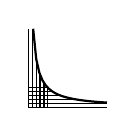
\begin{tikzpicture}[scale=0.25]
\draw(0,4)--(0,0)--(4,0);
\draw[thick,domain=0.25:4] plot(\x,1/\x);
\foreach\x in{0.2,0.4,...,1}\draw(\x,0)--(\x,{min(4,1/\x)});
\foreach\x in{0.2,0.4,...,1}\draw(0,\x)--({min(4,1/\x)},\x);
\end{tikzpicture}} &\sum_{k\leq a}\sum_{l\leq x/k}+\sum_{l\leq b}\sum - \sum\sum
\end{align*}
